\documentclass[12pt,a4paper]{article}
\usepackage[a4paper, margin=3cm]{geometry}
\usepackage{graphicx}
\usepackage{setspace}
% \usepackage{times}
\usepackage{ragged2e}
\usepackage{graphicx}
\usepackage{titling}
\usepackage{geometry}
\usepackage{listings}
\usepackage{xcolor}
\usepackage{float}
\usepackage{hyperref}
\usepackage{indentfirst}
\usepackage{setspace}
% \usepackage[natbibapa]{apacite}
\usepackage{natbib}

% ===== PHP & HTML Dark Theme Listing Style =====
\definecolor{codebg}{RGB}{30,30,46}
\definecolor{codetext}{RGB}{220,220,220}
\definecolor{phpkw}{RGB}{255,100,180}
\definecolor{phpstr}{RGB}{255,170,50}
\definecolor{phpfunc}{RGB}{255,215,70}
\definecolor{phpvar}{RGB}{255,150,210}
\definecolor{htmltagcol}{RGB}{80,210,210}
\definecolor{linenumcol}{RGB}{100,100,130}
\definecolor{commentcol}{RGB}{100,170,100}

\lstdefinestyle{phphtml}{
    backgroundcolor=\color{codebg},
    basicstyle=\ttfamily\small\color{codetext},
    breaklines=true,
    breakatwhitespace=true,
    tabsize=4,
    showstringspaces=false,
    numbers=left,
    numberstyle=\tiny\color{linenumcol},
    numbersep=10pt,
    frame=single,
    rulecolor=\color{gray!40},
    framesep=5pt,
    xleftmargin=18pt,
    % PHP language & keywords (pink/magenta)
    language=PHP,
    morekeywords={include, echo, while, if, else},
    keywordstyle=\color{phpkw}\bfseries,
    % Strings (orange)
    stringstyle=\color{phpstr},
    % Comments (green)
    commentstyle=\color{commentcol}\itshape,
    % Functions (yellow/gold)
    emph={mysqli_num_rows, mysqli_fetch_assoc, mysqli_close},
    emphstyle=\color{phpfunc},
    % Variables $... (pink)
    alsoletter={\$},
    emph={[2]\$result,\$row,\$koneksi},
    emphstyle={[2]\color{phpvar}},
    % HTML tags (cyan)
    moredelim=[s][\color{htmltagcol}\bfseries]{<}{>},
}
\usepackage{chngcntr}
\begin{document}

\begin{titlepage}
    \centering
    \onehalfspacing

    
    % Judul
    { \textbf{LAPORAN PRAKTIKUM}}\\[0.3cm]
    { \textbf{SISTEM ADMINISTRASI DAN INFORMASI TERDISTRIBUSI}}\\[0.3cm]
    { \textbf{PERTEMUAN 1}}\\[0.3cm]
    { \textbf{INSTALASI WEB SERVER DAN DATABASE DALAM KOMPUTER YANG BERBEDA}} \\[1.5cm]
    
    % Logo (ganti ugm.png dengan nama file logo kamu)
    
\includegraphics[height=7cm]{../images/ugm.png}
    
    % Identitas
    \begin{center}
Disusun oleh:\\[0.3cm]
\end{center}

\begin{center}
    \begin{tabular}{l c l}
        Nama & : & Hanan Fijananto \\
        NIM & : & 24/538946/SV/24555 \\
        Kelas & : & B2\\ 
        Dosen Pengampu & : & Dr.Imam Fahrurrozi, S.T., M.Cs.
    \end{tabular}
\end{center}


    
    \vspace{1.5cm}
    
    % Footer bawah
    { \textbf{PROGRAM STUDI D-IV TEKNOLOGI REKAYASA PERANGKAT LUNAK}}\\[0.3cm]
    { \textbf{DEPARTEMEN TEKNIK ELEKTRO DAN INFORMATIKA}}\\[0.3cm]
    { \textbf{SEKOLAH VOKASI}}\\[0.3cm]
    { \textbf{UNIVERSITAS GADJAH MADA}}\\[0.3cm]
    { \textbf{YOGYAKARTA}}\\[0.3cm]
    {\textbf{2026}}
    
\end{titlepage}

\doublespacing 

\section{Tujuan Praktikum}
\begin{enumerate}
    \item Mahasiswa mampu menginstalasi web server dan database dalam komputer yang berbeda.
    \item Mahasiswa mampu mengonfigurasi layanan MySQL pada server Linux agar dapat diakses dari komputer lain (modifikasi bind-address).
    \item Mahasiswa mampu mengonfigurasi layanan MySQL pada server Linux agar dapat diakses dari komputer lain (modifikasi user privileges).
\end{enumerate}

\section{Dasar Teori}
\section{Hasil dan Pemabahasan}
\subsection{Modifikasi bind-address pada MySQL}
Pada praktikum sebelumnya, Web Server Apache dan Database MySQL diinstal pada komputer yang sama. Pada praktikum ini, Web Server Apache dan Database MySQL diinstal pada komputer yang berbeda. Praktikan akan menggunakan komputer host untuk menginstall laragon untuk web server Apache serta VPS untuk database MySQL.

Untuk mengakses database MySQL yang terinstal pada VPS, praktikan perlu memodifikasi konfigurasi bind-address pada MySQL agar dapat menerima koneksi dari komputer lain. Berikut tahapannya:
\begin{enumerate}
    \item Buka VsCode yang sudah terhubung dengan VPS melalui SSH.
    \item Jalankan perintah berikut:
    \begin{lstlisting}[style=phphtml]
sudo nano /etc/mysql/mysql.conf.d/mysqld.cnf
    \end{lstlisting}
    \item Setelah dijalankan, akan muncul tampilan seperti berikut:
    \begin{figure}[H]
        \centering
        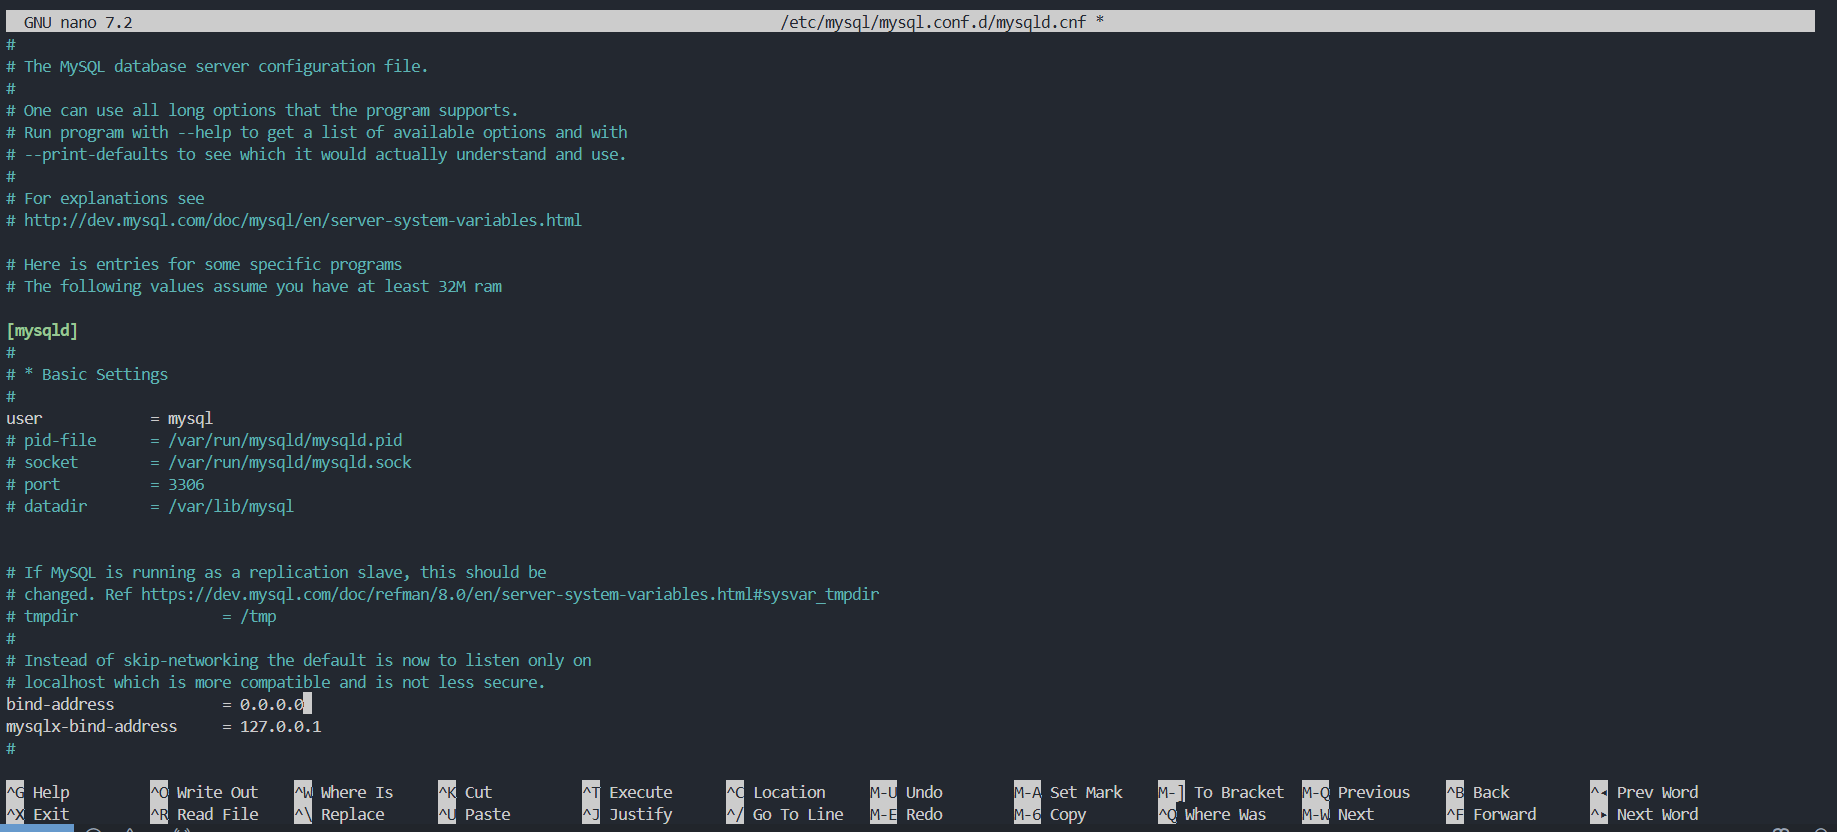
\includegraphics[width=0.8\textwidth]{../images/sudo-nano.png}
        \caption{Tampilan file mysqld.cnf}
    \end{figure}
    \item 
    \end{enumerate}
\subsection{Membuat User baru pada MySQL}

\subsection{}

\begin{lstlisting}[style=phphtml]
<?php

include 'tes_koneksi.php';

?>
<!DOCTYPE html>
<html>
<head>
    <title>Data Mahasiswa</title>
    <link rel="stylesheet" href="style.css">
</head>
<body>
<h2>Data Mahasiswa</h2>
<table>
    <tr>
        <th>ID</th>
        <th>NIM</th>
        <th>Nama</th>
        <th>Jurusan</th>
        <th>Angkatan</th>
        <th>Created At</th>
    </tr>
    <?php
    if (mysqli_num_rows($result) > 0) {
        while ($row = mysqli_fetch_assoc($result)) {
            echo "<tr>";
            echo "<td>" . $row['id'] . "</td>";
            echo "<td>" . $row['nim'] . "</td>";
            echo "<td>" . $row['nama'] . "</td>";
            echo "<td>" . $row['jurusan'] . "</td>";
            echo "<td>" . $row['angkatan'] . "</td>";
            echo "<td>" . $row['created_at'] . "</td>";
            echo "</tr>";
        }
    } else {
        echo "<tr><td colspan='6'>Tidak ada data</td></tr>";
    }

    mysqli_close($koneksi);
    ?>
</table>

</body>
</html>
\end{lstlisting}



\section{Kesimpulan}
\renewcommand{\refname}{\section{Daftar Pustaka}}
\bibliographystyle{IEEEtran}
\bibliography{ref}
\end{document}
